\section{Background}

% TODO: See how other people describe GP and BO}
In this section, we will present the problem formulation of analog circuit optimization, and review the background of Gaussian process regression and Bayesian optimization.

\subsection{Problem Formulation}

% TODO: The circuit performance comes from \bf{circuit} simulation}
% TODO: format, citation of HSPICE/spectre}
% TODO: See how other analog circuit optimization paper formulate the problem}

We handle the scenarios where the topology of the analog circuit is fixed. This
is practical as there are usually a lot of classical topologies for given
design task. Once the circuit topology is fixed, the designer has to choose the
appropriate design parameters according to the specifications and the circuit
device model. What we want to do is automatically searching for the optimal
design parameters. This problem can then be formulated as a bound-constrained
black-box optimization problem:
\begin{equation}
    \label{eq:Formulation}
    \text{minimize}~\mathrm{FOM}(\bm{x}),
\end{equation}
where $\bm{x} \in \textrm{D}$ is the vector of design variables,
$\mathrm{FOM}(\bm{x})$ is the objective constructed from the design
specifications. Given the design parameters $\bm{x}$, the FOM value can be
obtained by commercial circuit simulators like HSPICE or Spectre.

% \textcolor{red}{TODO: If there is still space, illustrate the objecive with the PM-width figure}

% \begin{figure}[]
%     \begin{center}
%         \centerline{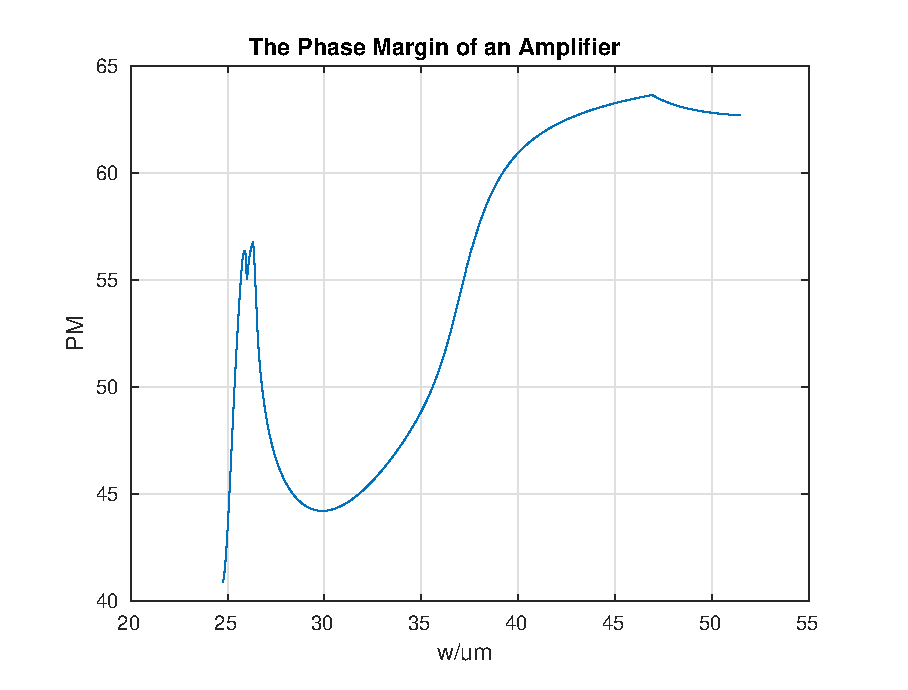
\includegraphics[width=\columnwidth]{./img/PM.eps}}
%         \caption{Phase margin of an amplifier as function of the width of a transistor}
%         \label{fig:PMOpAmp}
%     \end{center}
% \end{figure}

\subsection{Gaussian Process Regression}

\textcolor{red}{
    TODO:
    \begin{enumerate}
            \item Noise
            \item MLE learning
    \end{enumerate}
}

The objective function $\mathrm{FOM}(\bm{x})$ in \eqref{eq:Formulation} can be approximated by Gaussian
process (GP) model~\cite{GPML}. The GP model is the most commonly used model
for Bayesian optimization. The advantage of GP is that it provides a
well-calibrated uncertainty of prediction. GP is characterized by a mean
function $m(\bm{x})$ and a covariance function $k(\bm{x}, \bm{x'})$. In this
work, we use squared-exponential ARD kernel, and a constant mean function
$m(\bm{x}) = \mu_0$ for all our experiments.

Given a new data point $\bm{x}$, the prediction of $f(\bm{x})$ is
not a scalar value, but a predictive distribution
\begin{equation}
f(\bm{x}) \sim N(\mu(\bm{x}),
\sigma^2(\bm{x})),
\label{eq:GPRPred}
\end{equation}
where $\mu(\bm{x})$ and $\sigma^2(\bm{x})$ can be expressed as
\begin{equation}
        \begin{array}{lll}
            \mu(\bm{x}) &=& \mu_0 + k(\bm{x},X)K^{-1}(\bm{y} - \mu_0) \\
            \sigma^2(\bm{x}) &=&  - k(\bm{x}, X)K^{-1}k(X, \bm{x}),
        \end{array}
    \label{eq:GPRPredEqNoisy}
\end{equation}
where $k(\bm{x}, X) = (k(\bm{x}, \bm{x}_1), \dots, k(\bm{x},
\bm{x}_N))^T$ and $k(X, \bm{x}) = k(\bm{x}, X)^T$. The
$\mu(\bm{x})$ can be viewed as the prediction of the function value, while
the $\sigma^2(\bm{x})$ is a measure of uncertainty of the prediction. The hyperparameters including the parameters of the kernel function, and $\mu_0$ can be obtained by Maximum Likelihood Estimation (MLE) based on the training data set. 

\textcolor{red}{$\sigma_f$ ???, it is not necessary to mention it here.}

\subsection{Bayesian Optimization}

Bayesian optimization~\cite{shahriari2016taking} was proposed for the
optimization of expensive black-box functions. It consists of two essential
ingredients, i.e., the probabilistic surrogate models and the acquisition
functions. The probabilistic surrogate models provide predictions with
uncertainties. The acquisition functions make use of the predictive
distribution to explore the state space. The procedure of Bayesian optimization
is summarized in Algorithm~\ref{alg:BayesianOptAlgo}.


\begin{algorithm}
    \caption{Bayesian Optimization}
    \label{alg:BayesianOptAlgo}
    \begin{algorithmic}[1]
        \REQUIRE Number of initial sampling points $N_{init}$, number of iterations $N_{iter}$
        \STATE Randomly sample $N_{init}$ points in the design space
        \STATE Construct initial GP model
        \FOR{t = 1, 2, \dots, $N_{iter}$}
        \STATE Construct the acquisition function
        \STATE Find $\bm{x}_t$ that optimizes the acquisition function
        \STATE Sample $y_t = f(\bm{x}_t)$
        \STATE Update probabilistic surrogate model
        \ENDFOR
        \STATE \textbf{Return} best $f(\bm{x})$ recorded during iterations
    \end{algorithmic}
\end{algorithm}

In Bayesian optimization described in Algorithm~\ref{alg:BayesianOptAlgo}, the acquisition function is used to balance the exploration and exploitation during the optimization. The acquisition function considers both the predictive value and the uncertainty. There are a lot of existing acquisition functions. Examples include the lower confidence bound (LCB), the probability of improvement (PI), and the expected improvement (EI).

The LCB function is defined as follows:
\begin{equation}
    \label{eq:LCB}
    \mathrm{LCB}(\bm{x}) = \mu(\bm{x}) - \kappa \sigma(\bm{x}),
\end{equation}
where the $\mu(\bm{x})$ and the $\sigma(\bm{x})$ are the predictive value and uncertainty of GP, $\kappa$ is a parameter that balances the exploitation and exploration.

Following the suggestion of~\cite{brochu2010tutorial}, the $\kappa$ in \eqref{eq:LCB} is defined as:
\begin{equation}
    \label{eq:LCBKappa}
    \begin{array}{lll}
        \kappa &=& \sqrt{\nu \tau_t} \\
        \tau_t &=& 2 \log(t^{d/2+2} \pi^2 / 3 \delta),
    \end{array}
\end{equation}
where $t$ is the number of current iteration, $\nu$ and $\delta$ are two user-defined parameters. We fix $\nu = 0.5$ and $\delta = 0.05$ in this paper for the proposed MACE algorithm and our implementation of the BLCB algorithm.

The PI and EI functions are defined as
\begin{equation}
    \label{eq:PI_EI}
    \begin{array}{lll}
        \mathrm{PI}(\bm{x}) &=& \Phi(\lambda) \\
        \mathrm{EI}(\bm{x}) &=& \sigma(\bm{x}) (\lambda \Phi(\lambda) + \phi(\lambda))     \\
        \mathrm{\lambda}    &=& \displaystyle \frac{\tau - \xi - \mu(\bm{x})}{\sigma(\bm{x})},
    \end{array}
\end{equation}
where $\tau$ is the current best value objective value, and $\xi$ is a small positive jitter to improvement the ability of exploration. The $\Phi(.)$ and $\phi(.)$ functions are the CDF and PDF functions of normal distribution. We fix $\xi = 1e-3$ in our implementation of the MACE algorithm.

% TODO: discuss the different behaviours of LCB, EI, PI

There are also other acquisition functions, like the knowledge gradient~\cite{scott2011correlated} function, predictive entropy search~\cite{hernandez2014predictive}, and the max-value entropy search\cite{wang2017max}. A portfolio of several acquisition functions is also possible~\cite{hoffman2011portfolio}.
